\chapter{Results}

\section{Environmental and spatial drivers of \textit{Parthenium hysterophorus} presence in Pakistan}

\subsection{Model selection}

Model selection showed that incorporating spatial structure substantially improved model performance (Table~\ref{tab:model-comparison}). The non-spatial model (M1\_noloc) explained just 38.17\% of the deviance and had the poorest fit, with an AIC 1678.86 units higher than the best-performing model. In contrast, models with a two-dimensional spatial smooth explained 55.37\% to 60.33\% of the deviance, highlighting the importance of spatial dependence.

Among REML-fitted models, increasing the spatial smooth basis from $k = 100$ (M4\_k100) to $k = 200$ (M5\_k200) produced the best model, reducing AIC by 207.83 units and raising explained deviance from 56.82\% to 60.33\%. Excluding altitude (M3\_xalt) substantially reduced model performance (AIC increased by 314.69 units; deviance explained fell to 55.37\%), demonstrating altitude's unique explanatory value beyond climatic and spatial predictors. Maximum-likelihood comparisons further supported retaining road type in the final model. Excluding road type (M7\_noroad) or its smooth interaction (M6\_noroad\_sm) significantly reduced model fit compared to the full model (M8\_full\_ml), with AIC increases of 19.04 units or more ($p < 0.001$). Thus, M5\_k200 was selected for further analyses, as it minimised AIC, maximised explanatory power, and included all ecologically relevant predictors.

Although basis-dimension diagnostics yielded $k$-index values below one for all spatial models (0.72--0.80; $p < 0.001$), increasing $k$ to 200 substantially improved model performance, justifying its use in the final model. A substantial residual spatial component remained after accounting for environmental, habitat, and road variables. The spatial Gaussian-process smooth was highly significant (edf = 109.80, $\chi^2$ = 977.85, $p < 0.001$), indicating spatial structure in occurrence beyond measured environmental predictors. Therefore, the spatial term was retained to account for geographically structured variation in occurrence rather than as an environmental driver.

\begin{table}[H]
    \centering
    \caption{Model comparison and goodness-of-fit evaluation across generalised additive model (GAM) candidate formulations. Models are fitted via Restricted Maximum Likelihood (REML) and evaluated based on Total Effective Degrees of Freedom (EDF), percentage deviance explained, Akaike Information Criterion (AIC), change in AIC relative to the best-performing model ($\Delta\text{AIC}$), likelihood-ratio test (LRT) $p$-values, and spatial basis-dimension adequacy ($k$-index and $p$-value from \texttt{k.check}). The primary full model (M5\_k200) is retained in red.}
    \label{tab:model-comparison}
    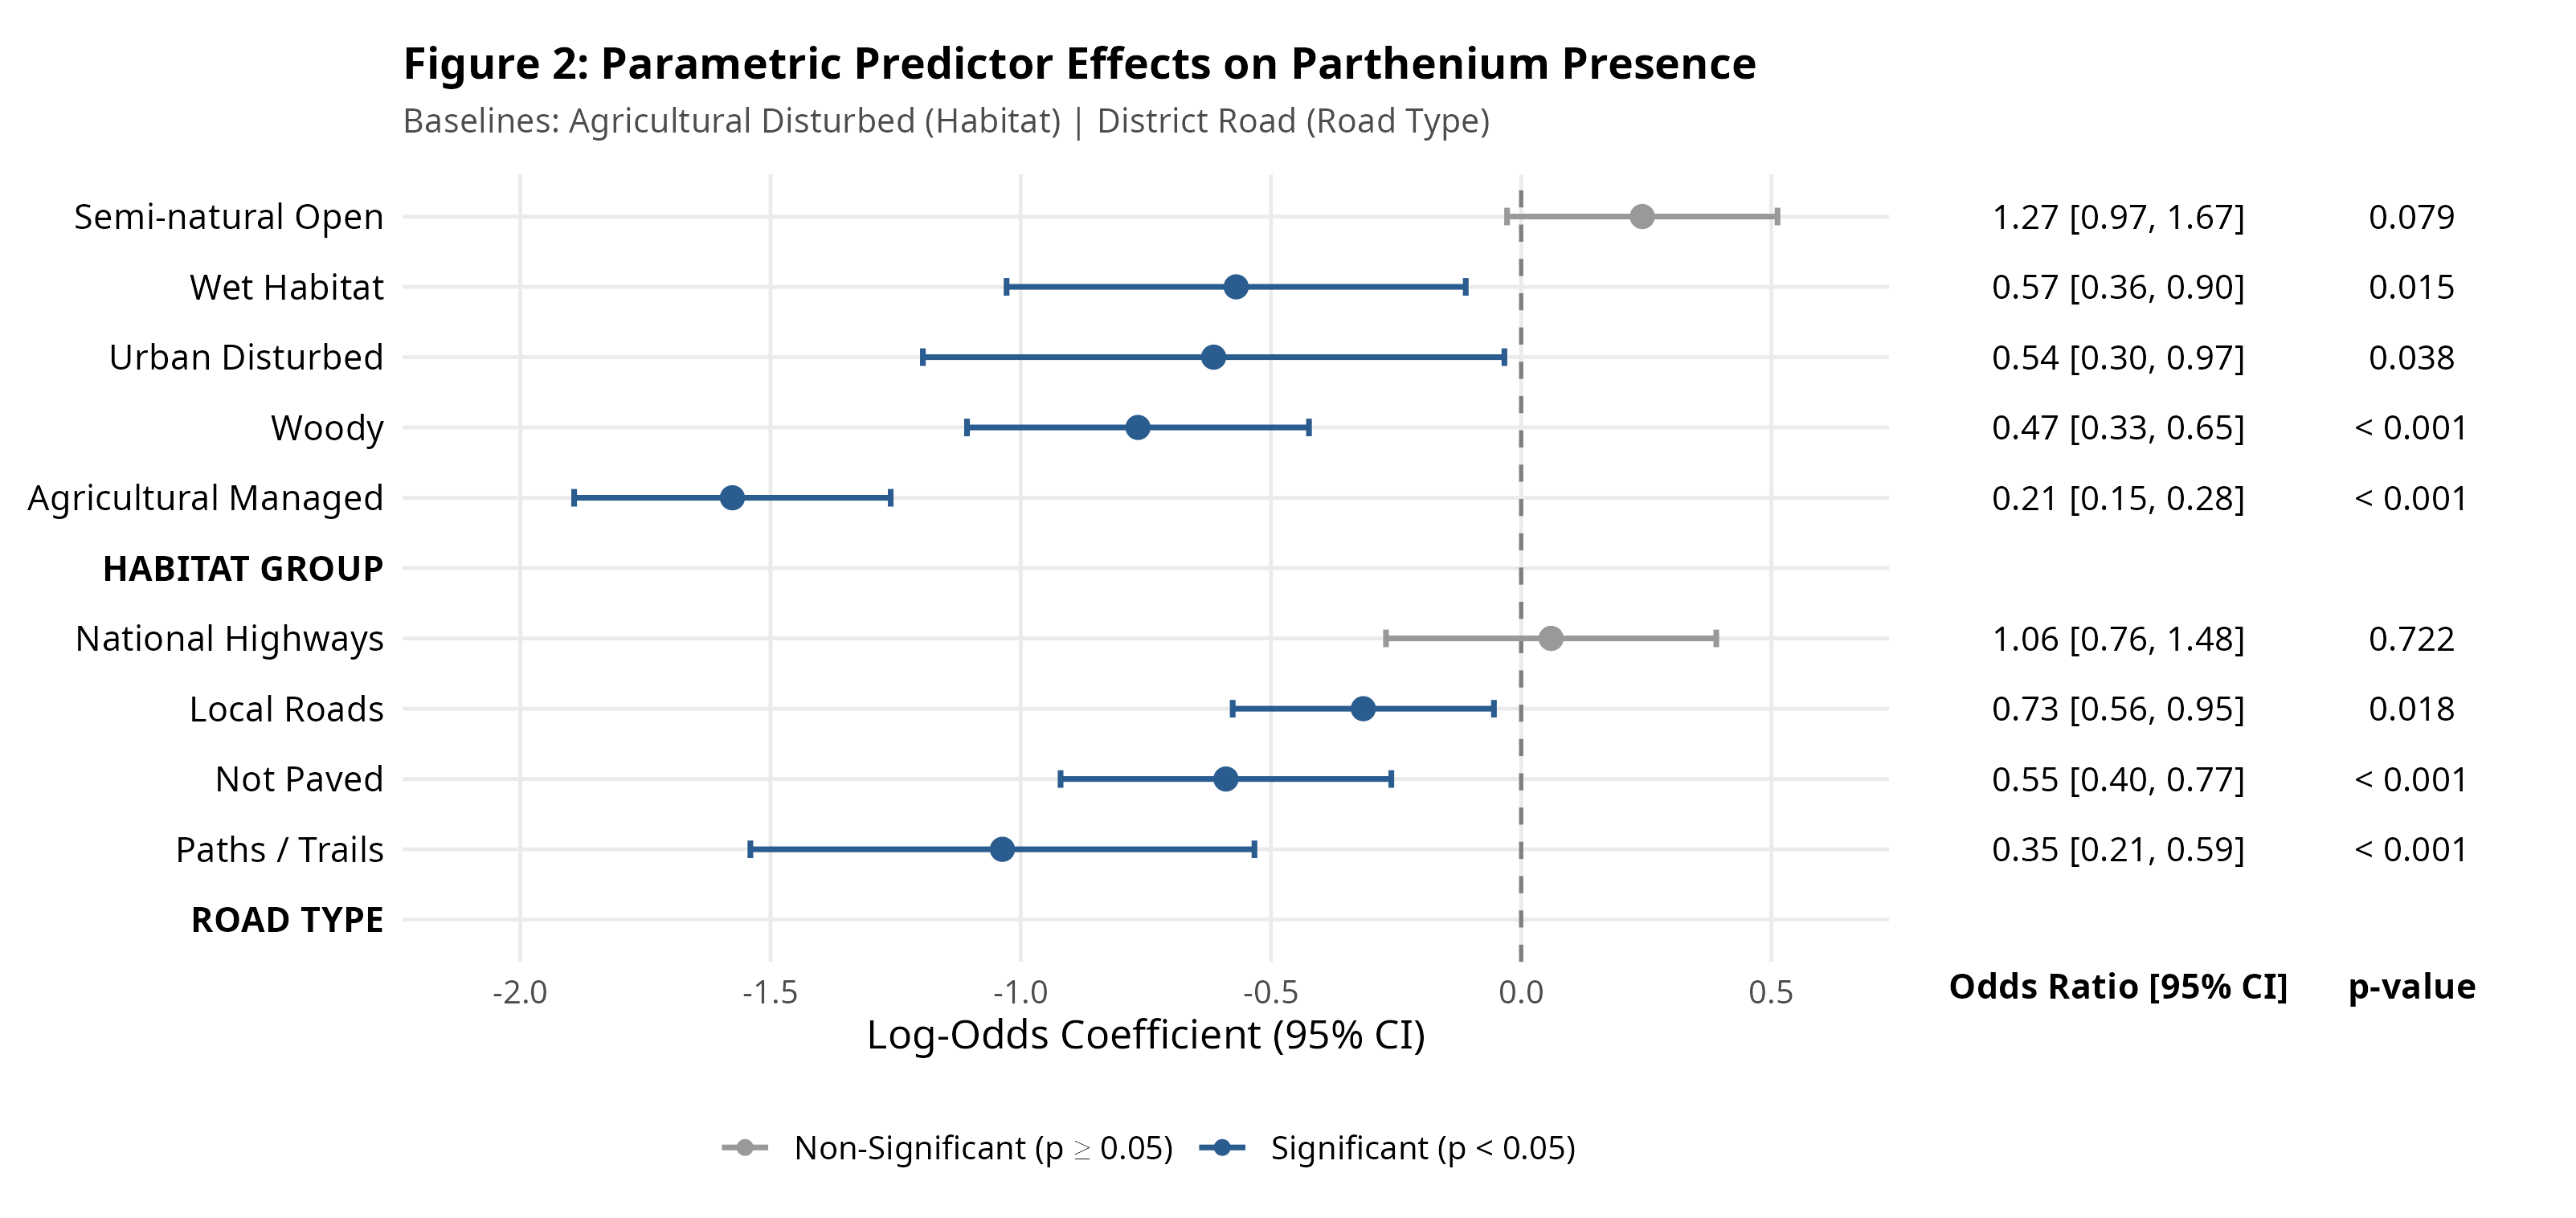
\includegraphics[width=\textwidth]{figures/fig2_parametric_forest_table.png}
\end{table}

\subsection{Final model performance}

The final REML-fitted GAM explained 60.33\% of the deviance in \textit{Parthenium hysterophorus} presence (adjusted $R^2 = 0.629$, REML = 2000.6, $n = 6{,}852$). The model included a bivariate spatial smooth (longitude, latitude), global smooths for cumulative temperature and growing degree days (GDD), habitat-specific smooths for GDD, altitude, habitat cover, habitat group, and road type.

The final model can be expressed as:

\begin{verbatim}
gam_gdd_k_200 <- gam(
  presence ~
    hab_group +
    road_type +
    s(precip_sum_30d, k = 25) +
    s(gdd_30d, k = 25) +
    s(gdd_30d, by = hab_group, k = 15) +
    s(altitude, k = 15) +
    s(hab_perc, k = 10) +
    s(longitude, latitude, bs = "gp", k = 200),
  family = binomial(link = "logit"),
  method = "REML",
  data = survey_data)
\end{verbatim}

Further analyses assessed the significance and functional form of smooth and parametric terms to identify key environmental and spatial drivers of \textit{P. hysterophorus} occurrence in Pakistan.

\section{Parametric effects of habitat and transport infrastructure}

Parametric fixed effects from the final GAM (M5\_k200) showed significant variation in \textit{P. hysterophorus} occurrence odds across habitat groups and road types (Figure~\ref{fig:parametric-effects}). Coefficients are reported as log-odds and odds ratios, relative to the Agricultural Disturbed habitat and District Road reference categories.

\subsection*{Habitat group}

Habitat group strongly influenced occurrence odds. All categories except Semi-natural Open differed significantly from the Agricultural Disturbed baseline ($p < 0.05$):

\begin{itemize}
    \item Semi-natural Open habitat had a positive but non-significant difference from disturbed agriculture ($\beta = 0.237$, SE = 0.138, $p = 0.084$), indicating similar or slightly higher occurrence probability in unmanaged open areas.
    \item Urban Disturbed ($\beta = -0.599$, OR = 0.55, $p = 0.043$), Wet Habitat ($\beta = -0.580$, OR = 0.56, $p = 0.013$), and Woody Vegetation ($\beta = -0.772$, OR = 0.46, $p < 0.001$) all showed significantly reduced odds of occurrence.
    \item Agricultural Managed land had the strongest negative effect, reducing occurrence odds by 79\% compared to disturbed agriculture ($\beta = -1.569$, OR = 0.21, $p < 0.001$).
\end{itemize}

\subsection*{Road type}

Occurrence odds declined along a gradient of decreasing road size, traffic volume, and accessibility (Figure~\ref{fig:parametric-effects}):

\begin{itemize}
    \item National Highways did not differ significantly from District Roads ($\beta = 0.039$, OR = 1.04, $p = 0.814$), indicating high occurrence probability along both major transport corridors.
    \item Lower-tier routes showed reduced occurrence odds: Local Roads ($\beta = -0.340$, OR = 0.71, $p = 0.010$) and Unpaved Roads ($\beta = -0.612$, OR = 0.54, $p < 0.001$).
    \item Paths and Trails had the largest reduction, lowering odds by 66\% compared to District Roads ($\beta = -1.077$, OR = 0.34, $p < 0.001$).
\end{itemize}

These results reveal a clear disturbance gradient: occurrence odds are highest in habitats and road types with the most disturbance and vehicular traffic (District Roads, National Highways, Agricultural Disturbed, Semi-natural Open). Odds decrease with greater disturbance suppression (Agricultural Managed, Woody habitat) or lower propagule delivery (Local, Unpaved Roads, Paths/Trails). This pattern aligns with the established ecology of \textit{P. hysterophorus} as a ruderal and disturbance-dependent species and supports the role of road networks and land management as primary drivers of \textit{P. hysterophorus} occurrence.

\begin{figure}[H]
    \centering
    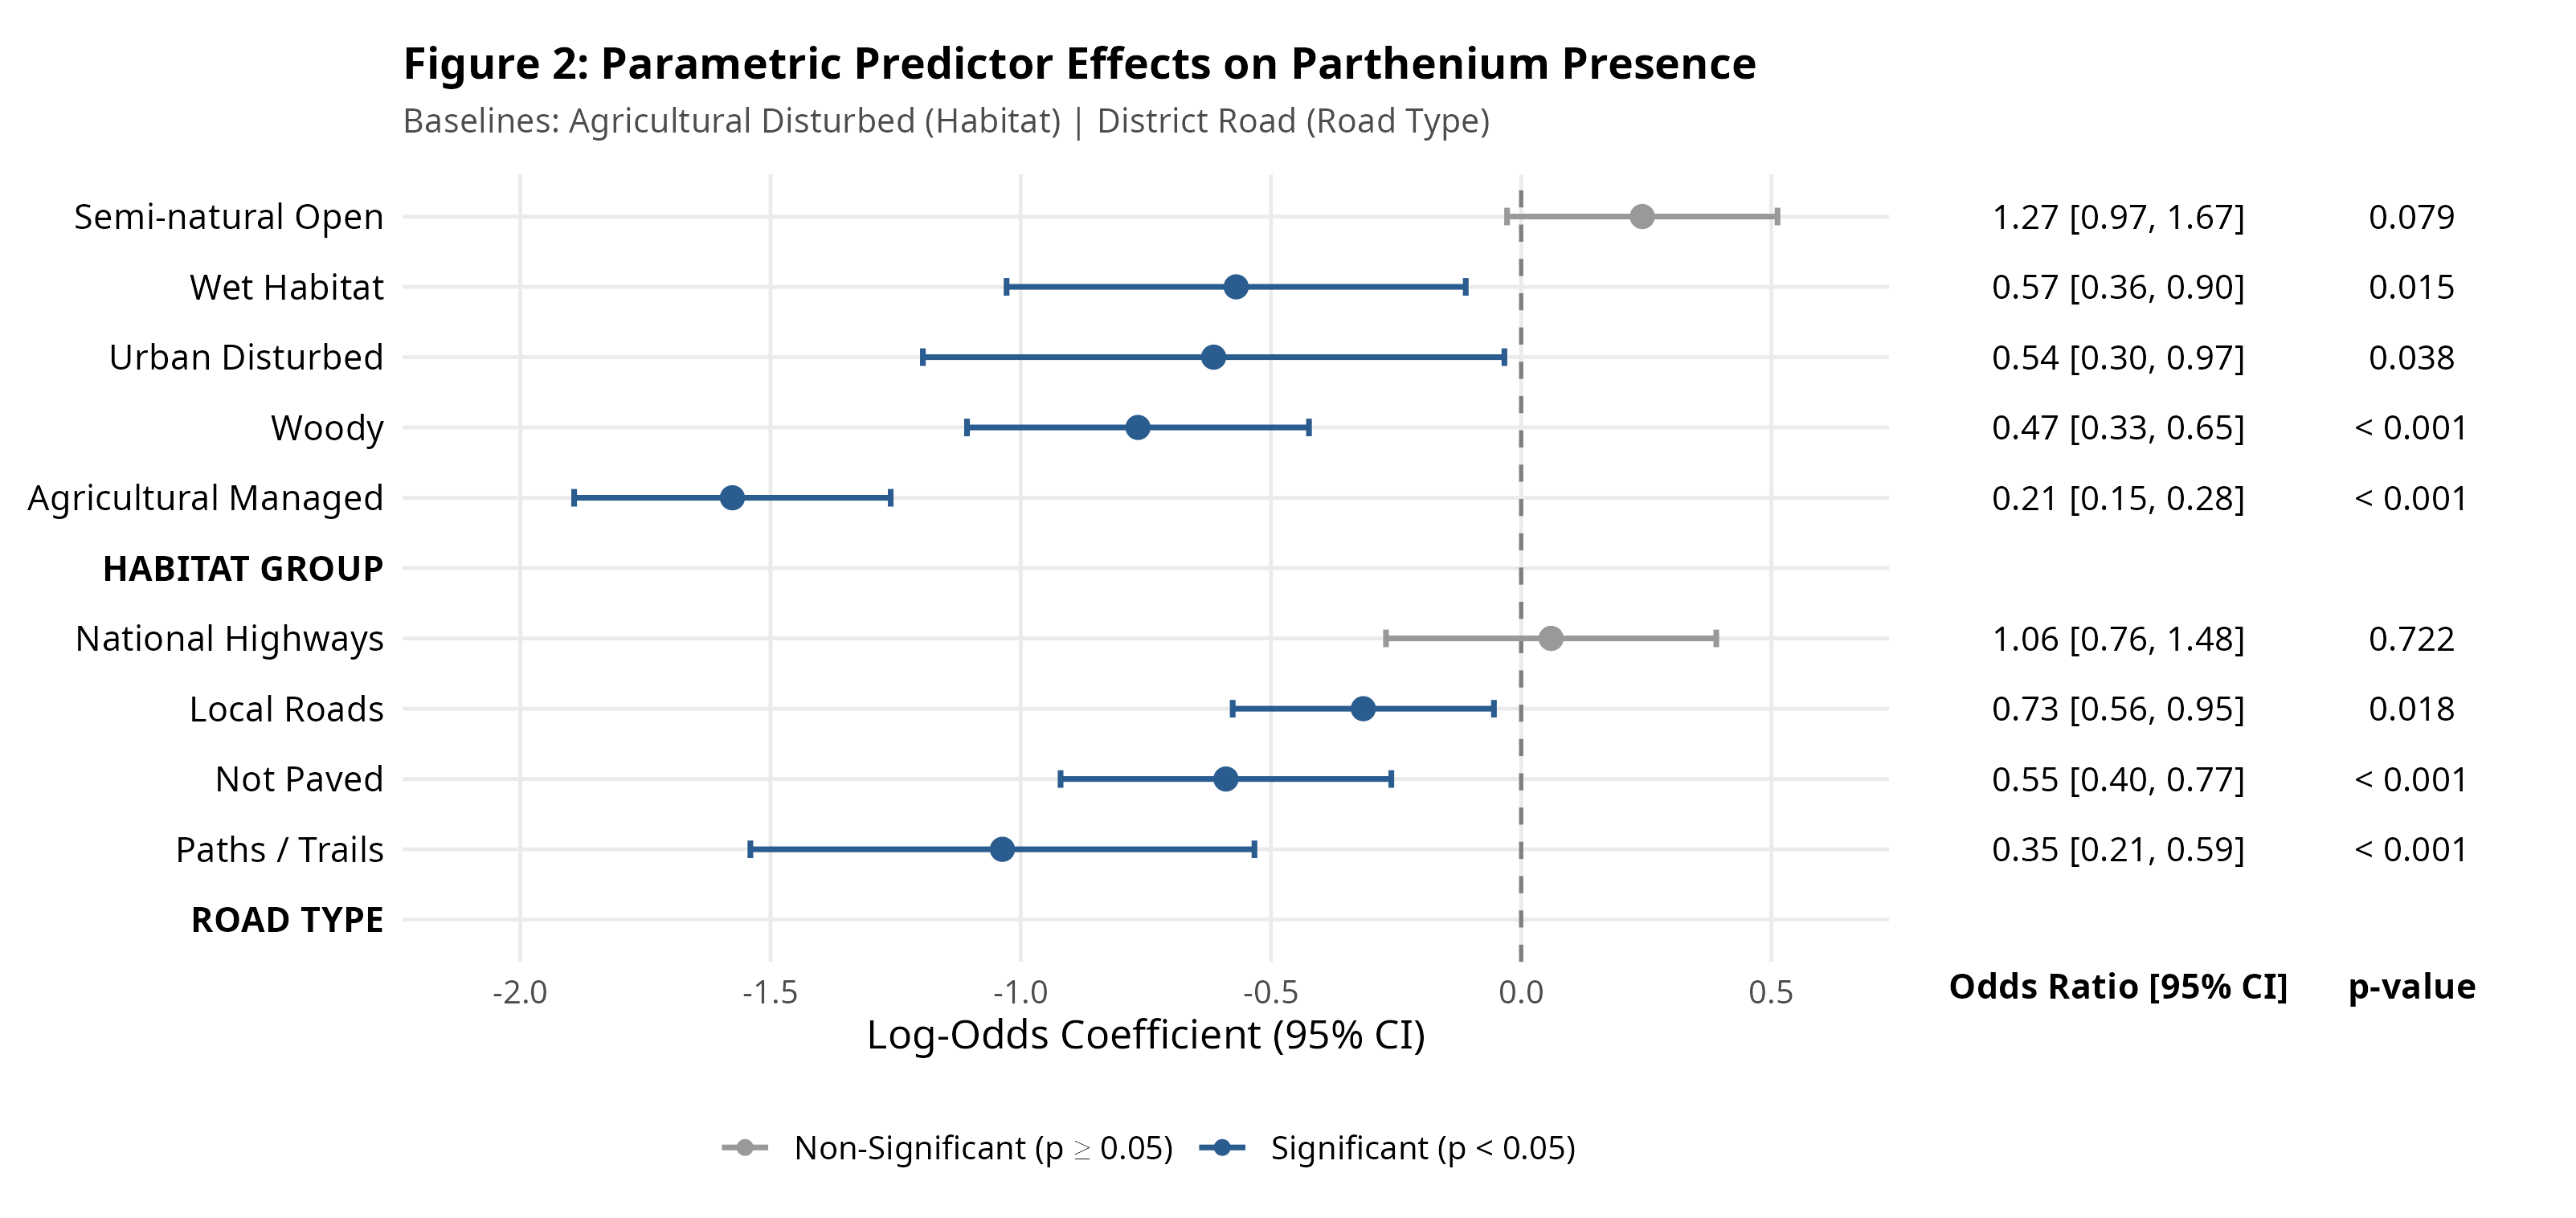
\includegraphics[width=\textwidth]{figures/fig2_parametric_forest_table.png}
    \caption{Parametric fixed effects on \textit{Parthenium hysterophorus} occurrence. Left panel: forest plot of log-odds coefficients (95\% confidence intervals) relative to baseline reference categories (Agricultural Disturbed for habitat; District Road for road classification). Points and error bars are colored by statistical significance (alpha = 0.05). Right panel: corresponding exponentiated odds ratios (OR = $e^{\beta}$) with 95\% confidence intervals and two-tailed $p$-values.}
    \label{fig:parametric-effects}
\end{figure}

\section{Non-linear climate responses across habitat types}

\subsection*{Regional thermal response: growing degree days (GDD)}

Growing degree days over the preceding 30 days (30dGDD) were a strong, non-linear predictor of \textit{Parthenium hysterophorus} occurrence. The global smooth was highly significant (edf = 11.51, $\chi^2$ = 81.26, $p < 0.001$), with diagnostics ($k' = 24$, $k$-index = 0.99) supporting genuine non-linearity rather than a modelling artefact.

Predicted occurrence was highest in Semi-natural Open and Agricultural Disturbed habitats and lowest in Agricultural Managed land, particularly across 200--750 30dGDD. In the less-managed habitats, occurrence probability peaked around 300 and 650--700 30dGDD (0.25--0.30), whereas Agricultural Managed habitats showed near-zero probability across the gradient (Figure~\ref{fig:gdd-response}).

Raw observations similarly indicated elevated occurrence at 50--150, 450--500, and particularly 600--750 30dGDD, followed by a decline above 750. However, sparse sampling at the gradient extremes and wide confidence intervals limit interpretation of these apparent peaks as biological thresholds.

Occurrence also varied seasonally, with presence rates highest in August and additional increases in November in some habitats, while February--March and October were lower. This pattern suggests the GDD response reflects seasonal phenology and habitat conditions rather than multiple physiological optima. Overall, 30dGDD was an important predictor, but occurrence is likely also shaped by precipitation, soil moisture, disturbance, vegetation structure, and land management.

\begin{figure}[H]
    \centering
    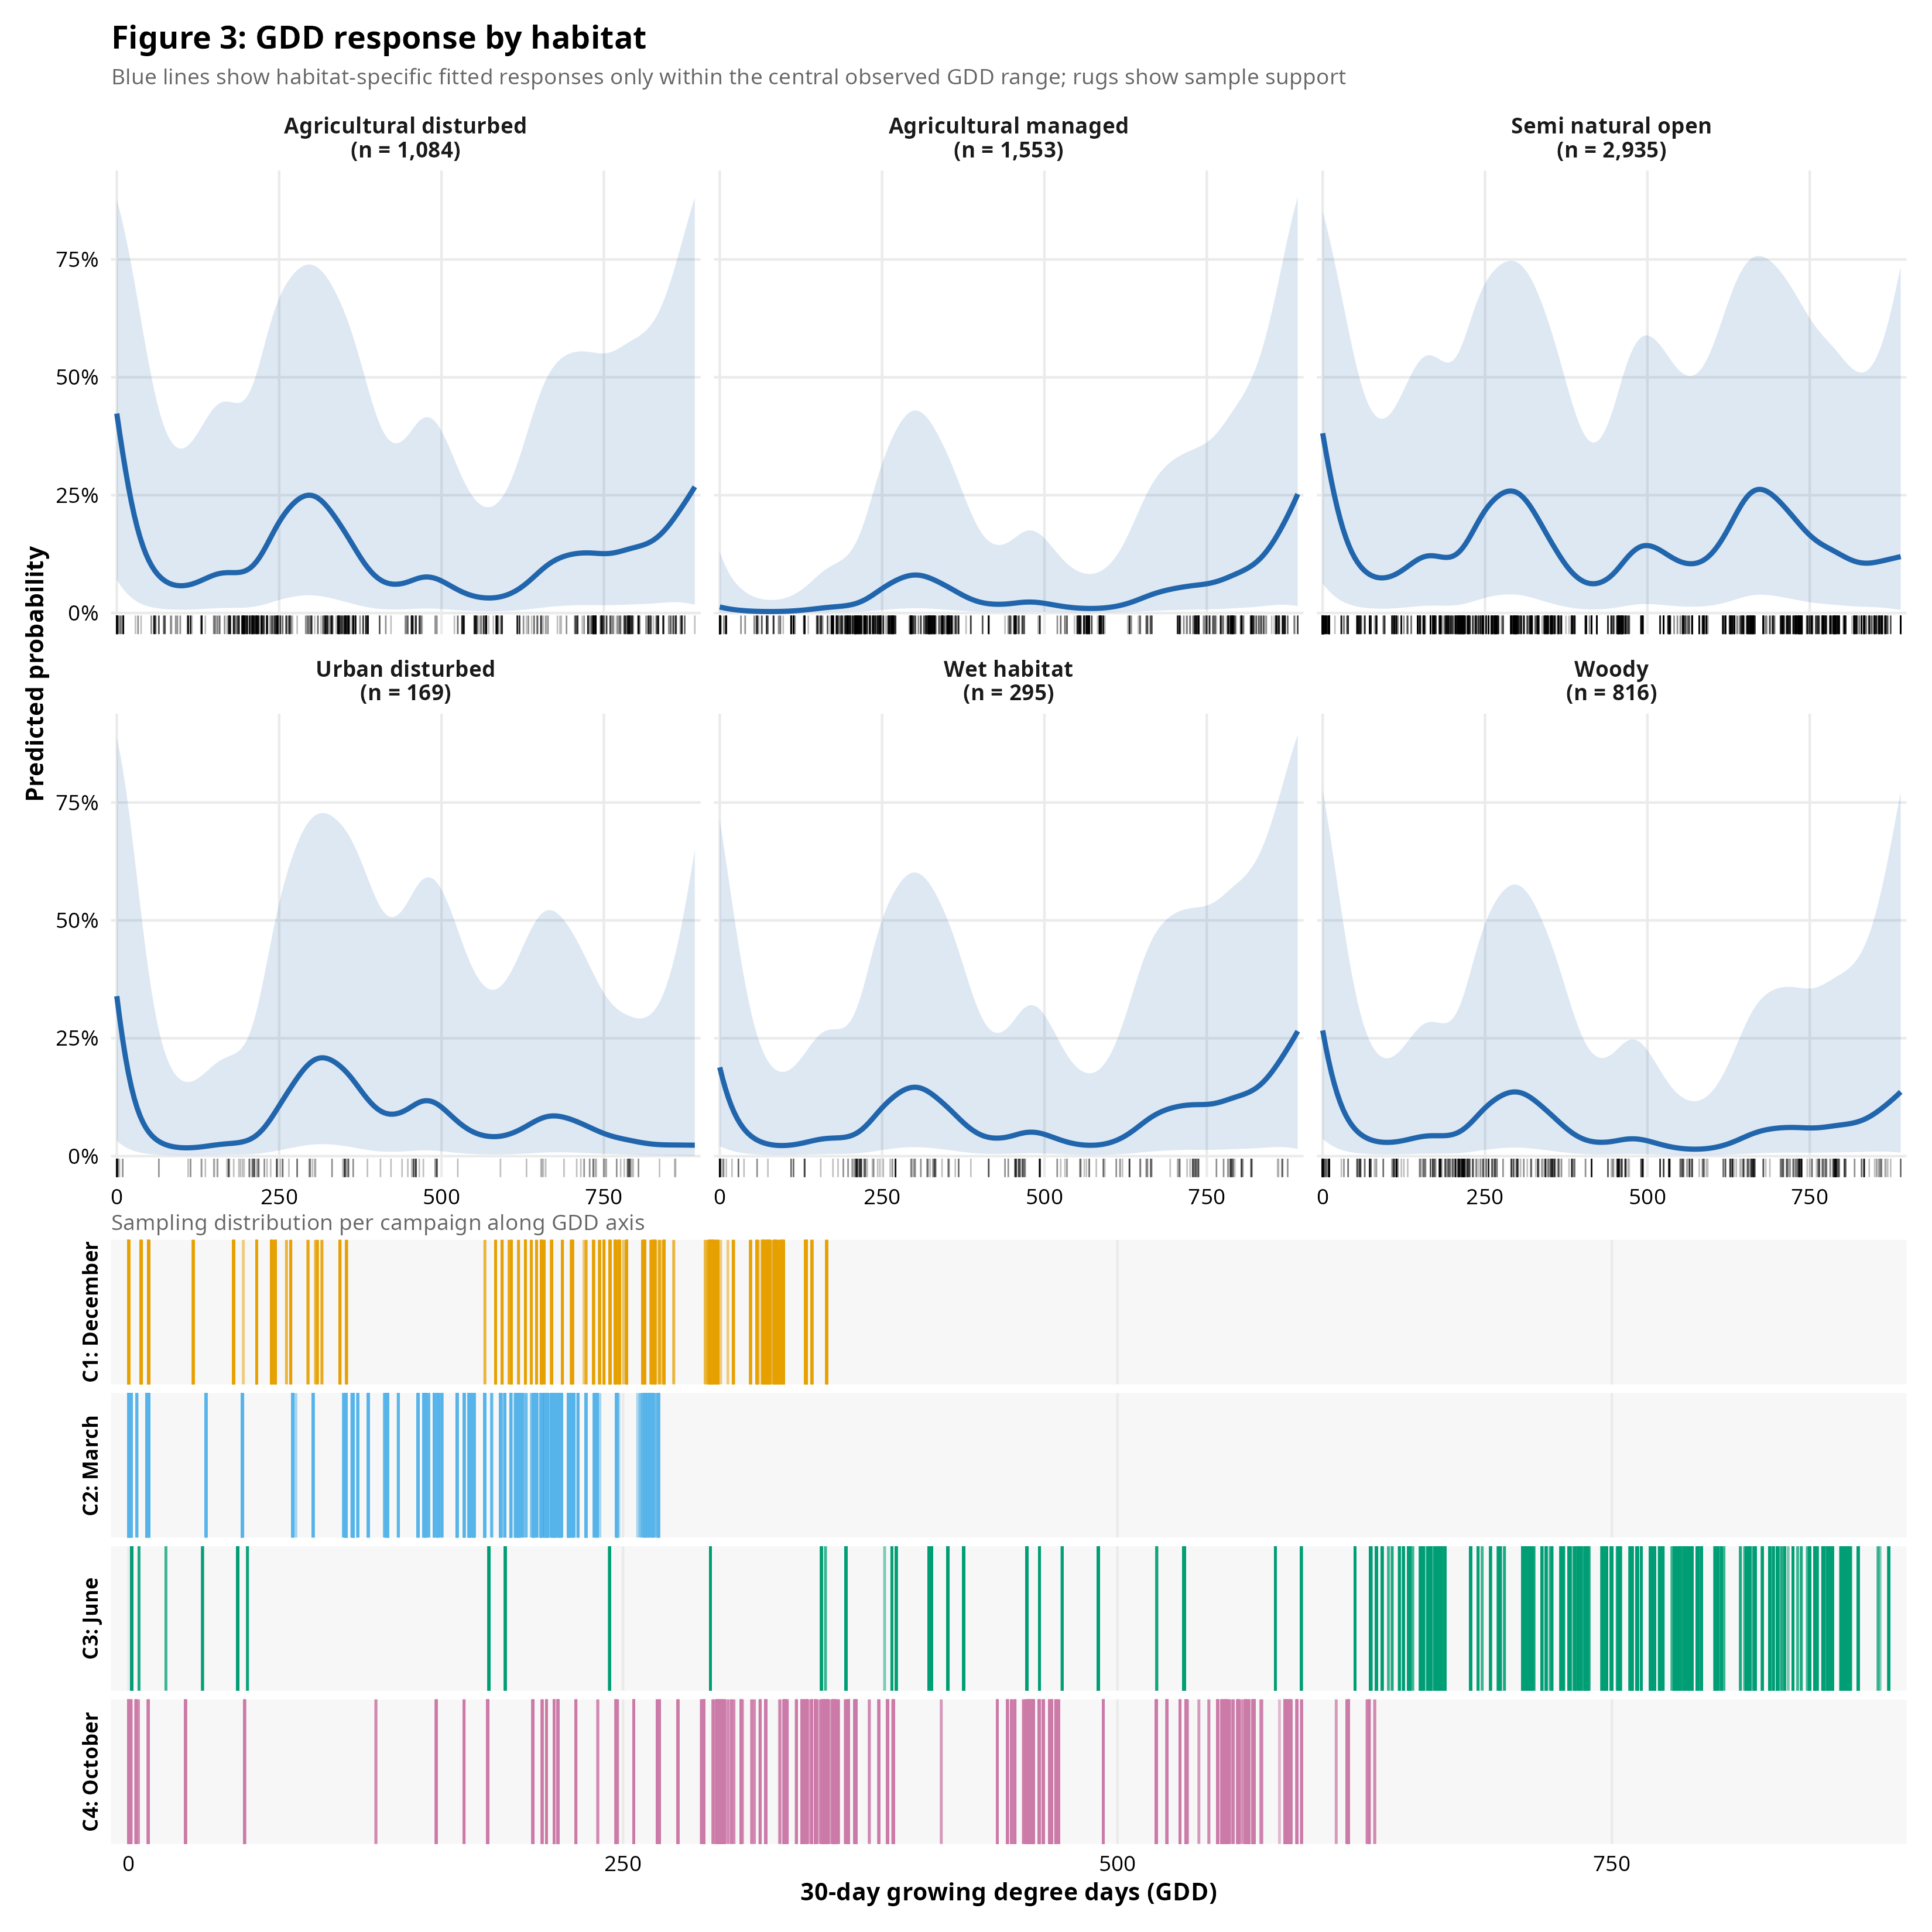
\includegraphics[width=\textwidth]{figures/fig3_with_campaign_rug.png}
    \caption{Non-linear response of \textit{Parthenium hysterophorus} occurrence probability to 30-day Growing Degree Days ($\text{GDD}_{30\text{d}}$) across habitat groups. Curves depict partial predictions from model \texttt{M5\_k200} holding spatial and secondary predictors constant. Shaded ribbons represent 95\% confidence intervals. Note that sharp probability increases and wide confidence ribbons at boundary extremes ($\text{GDD}_{30\text{d}} < 50$ and $> 800$) reflect sparse sampling density and spline boundary uncertainty.}
    \label{fig:gdd-response}
\end{figure}

\subsection*{Precipitation and other environmental predictors}

The relationship between 30-day cumulative precipitation and occurrence was nonlinear and highly significant (edf = 4.59, $\chi^2$ = 28.56, $p < 0.001$). Occurrence probability was highest at low to moderate precipitation, peaking at 50--120 mm and plateauing near 100 mm ($\approx 0.23$). As precipitation increased, probability declined, with greater uncertainty at the upper end of the range (Figure~\ref{fig:precip-response}).

Beyond 120 mm, occurrence probability declined sharply, approaching zero above 200 mm. This pattern matches the categorical habitat effect, with wet habitats showing lower occurrence than agricultural disturbed areas. Overall, moisture availability emerged as a key environmental correlate of \textit{P. hysterophorus} occurrence.

At very low precipitation ($< 25$ mm), the response curve rose slightly and confidence intervals widened, likely due to sparse sampling and hydrological effects such as irrigation or drainage. Altitude also showed a strong association with occurrence (edf = 5.25, $\chi^2$ = 56.94, $p < 0.001$), while habitat cover had a weaker but significant nonlinear effect (edf = 2.00, $\chi^2$ = 8.99, $p = 0.017$).

\begin{figure}[H]
    \centering
    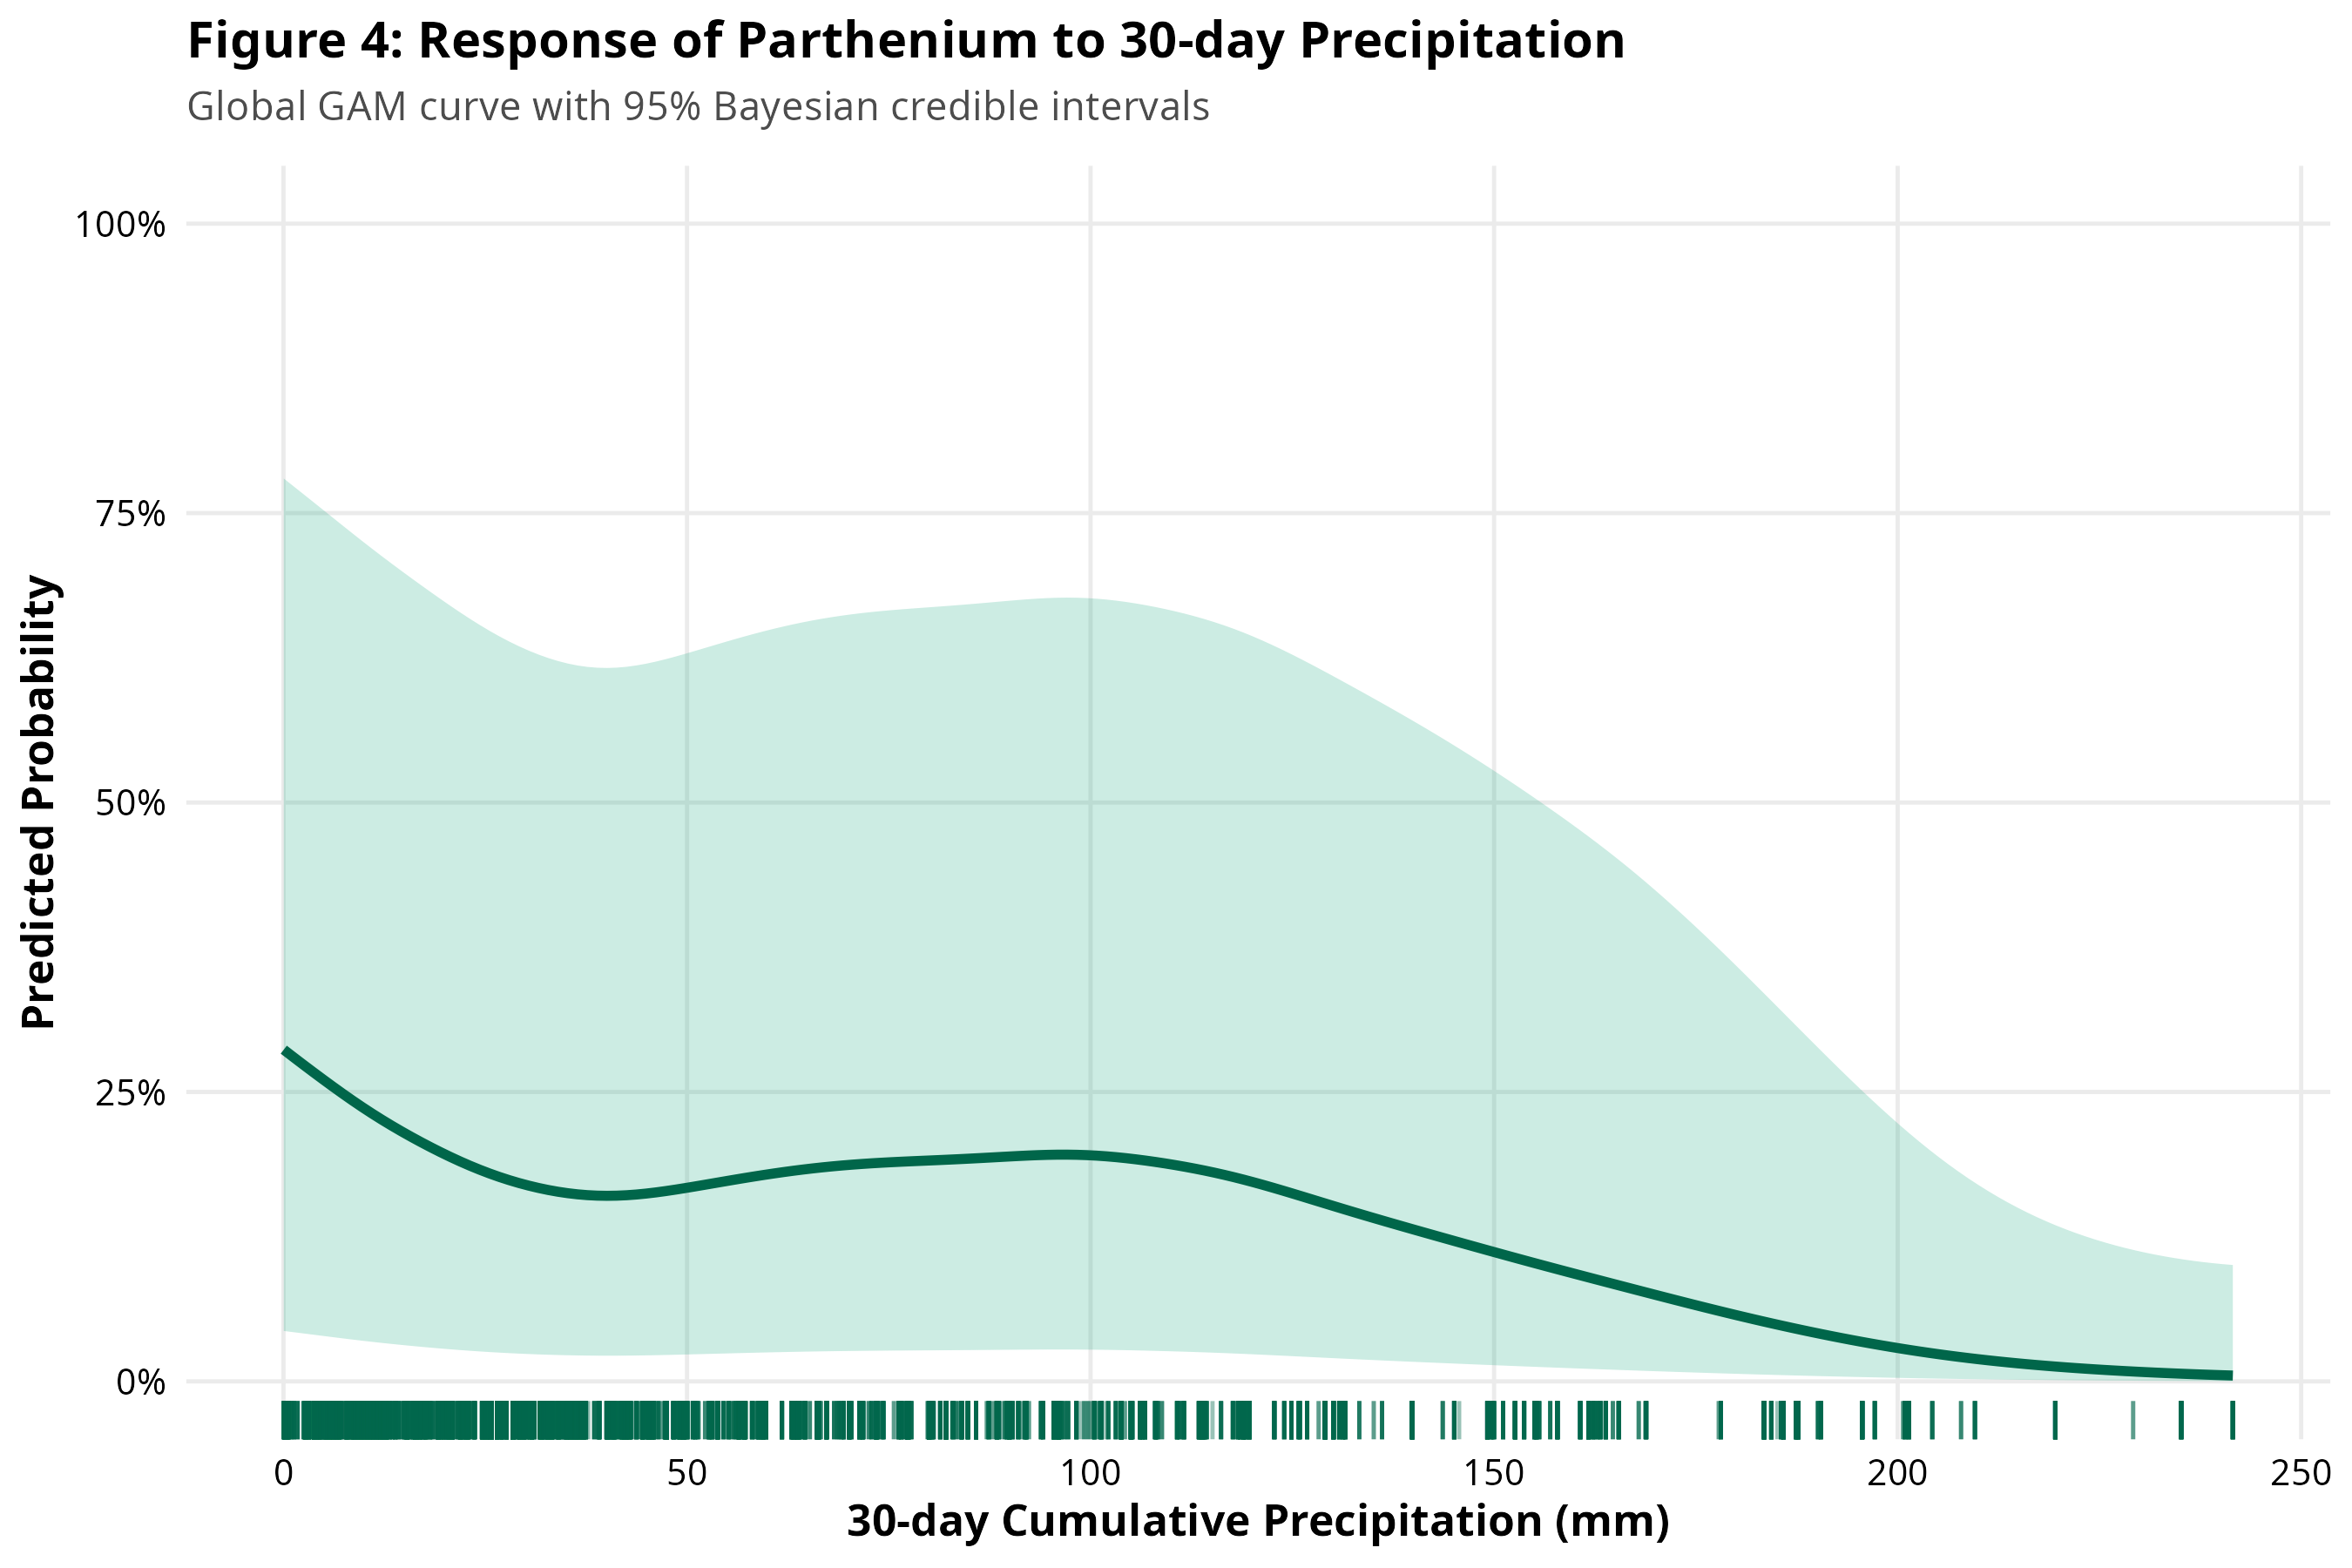
\includegraphics[width=\textwidth]{figures/fig4_precipitation_smooth.png}
    \caption{Partial response curve of \textit{Parthenium hysterophorus} occurrence probability to 30-day cumulative precipitation (mm). The solid line represents the expected partial smooth effect from model \texttt{M5\_k200} with secondary covariates held constant; the shaded ribbon depicts 95\% confidence intervals. Widened confidence bands at low precipitation thresholds ($< 25$ mm) reflect domain edge uncertainty and sparse observation density.}
    \label{fig:precip-response}
\end{figure}

\section{Forecasting and biocontrol thermal suitability (India, 2030/2050)}

Figure~\ref{fig:india-projections} presents projected climatic suitability for \textit{Parthenium hysterophorus}, the thermal suitability proxy for \textit{Zygogramma bicolorata}, and their spatial overlap across India under present, 2030, and 2050 climate scenarios. A lower \textit{Parthenium} threshold was used to capture marginally suitable areas that may represent early-warning invasion pathways. The \textit{Zygogramma} layer represents broad thermal-climatic permissiveness rather than direct predictions of beetle establishment or biocontrol efficacy.

MaxEnt projections indicated that \textit{Parthenium} suitability is extensive under current conditions but becomes increasingly restricted and fragmented under future scenarios. In contrast, the annual temperature-based \textit{Zygogramma} proxy remained high across most of India, indicating persistent annual thermal permissiveness despite warming. Using thresholds of 0.4952 for \textit{Parthenium} and 0.75 for \textit{Zygogramma}, jointly suitable cells declined from 66.0\% under current conditions to 42.0\% in 2030 and 20.6\% in 2050. Beetle-only cells increased from 30.4\% to 55.8\% and 77.5\%, respectively, while \textit{Parthenium}-only cells remained negligible. Thus, declining overlap was primarily driven by contraction of \textit{Parthenium} suitability rather than loss of annual beetle thermal suitability.

Despite the permissive \textit{Parthenium} threshold, future climate projections did not produce a broad national-scale area where \textit{Parthenium} suitability exceeded the beetle proxy. However, the 2050 summer heat-stress panel provides an important seasonal contrast: although annual conditions remain broadly permissive for \textit{Zygogramma}, large areas may experience temperatures approaching or exceeding its upper thermal limits. This indicates that seasonal heat stress may impose constraints not captured by the annual thermal proxy.

\begin{figure}[H]
    \centering
    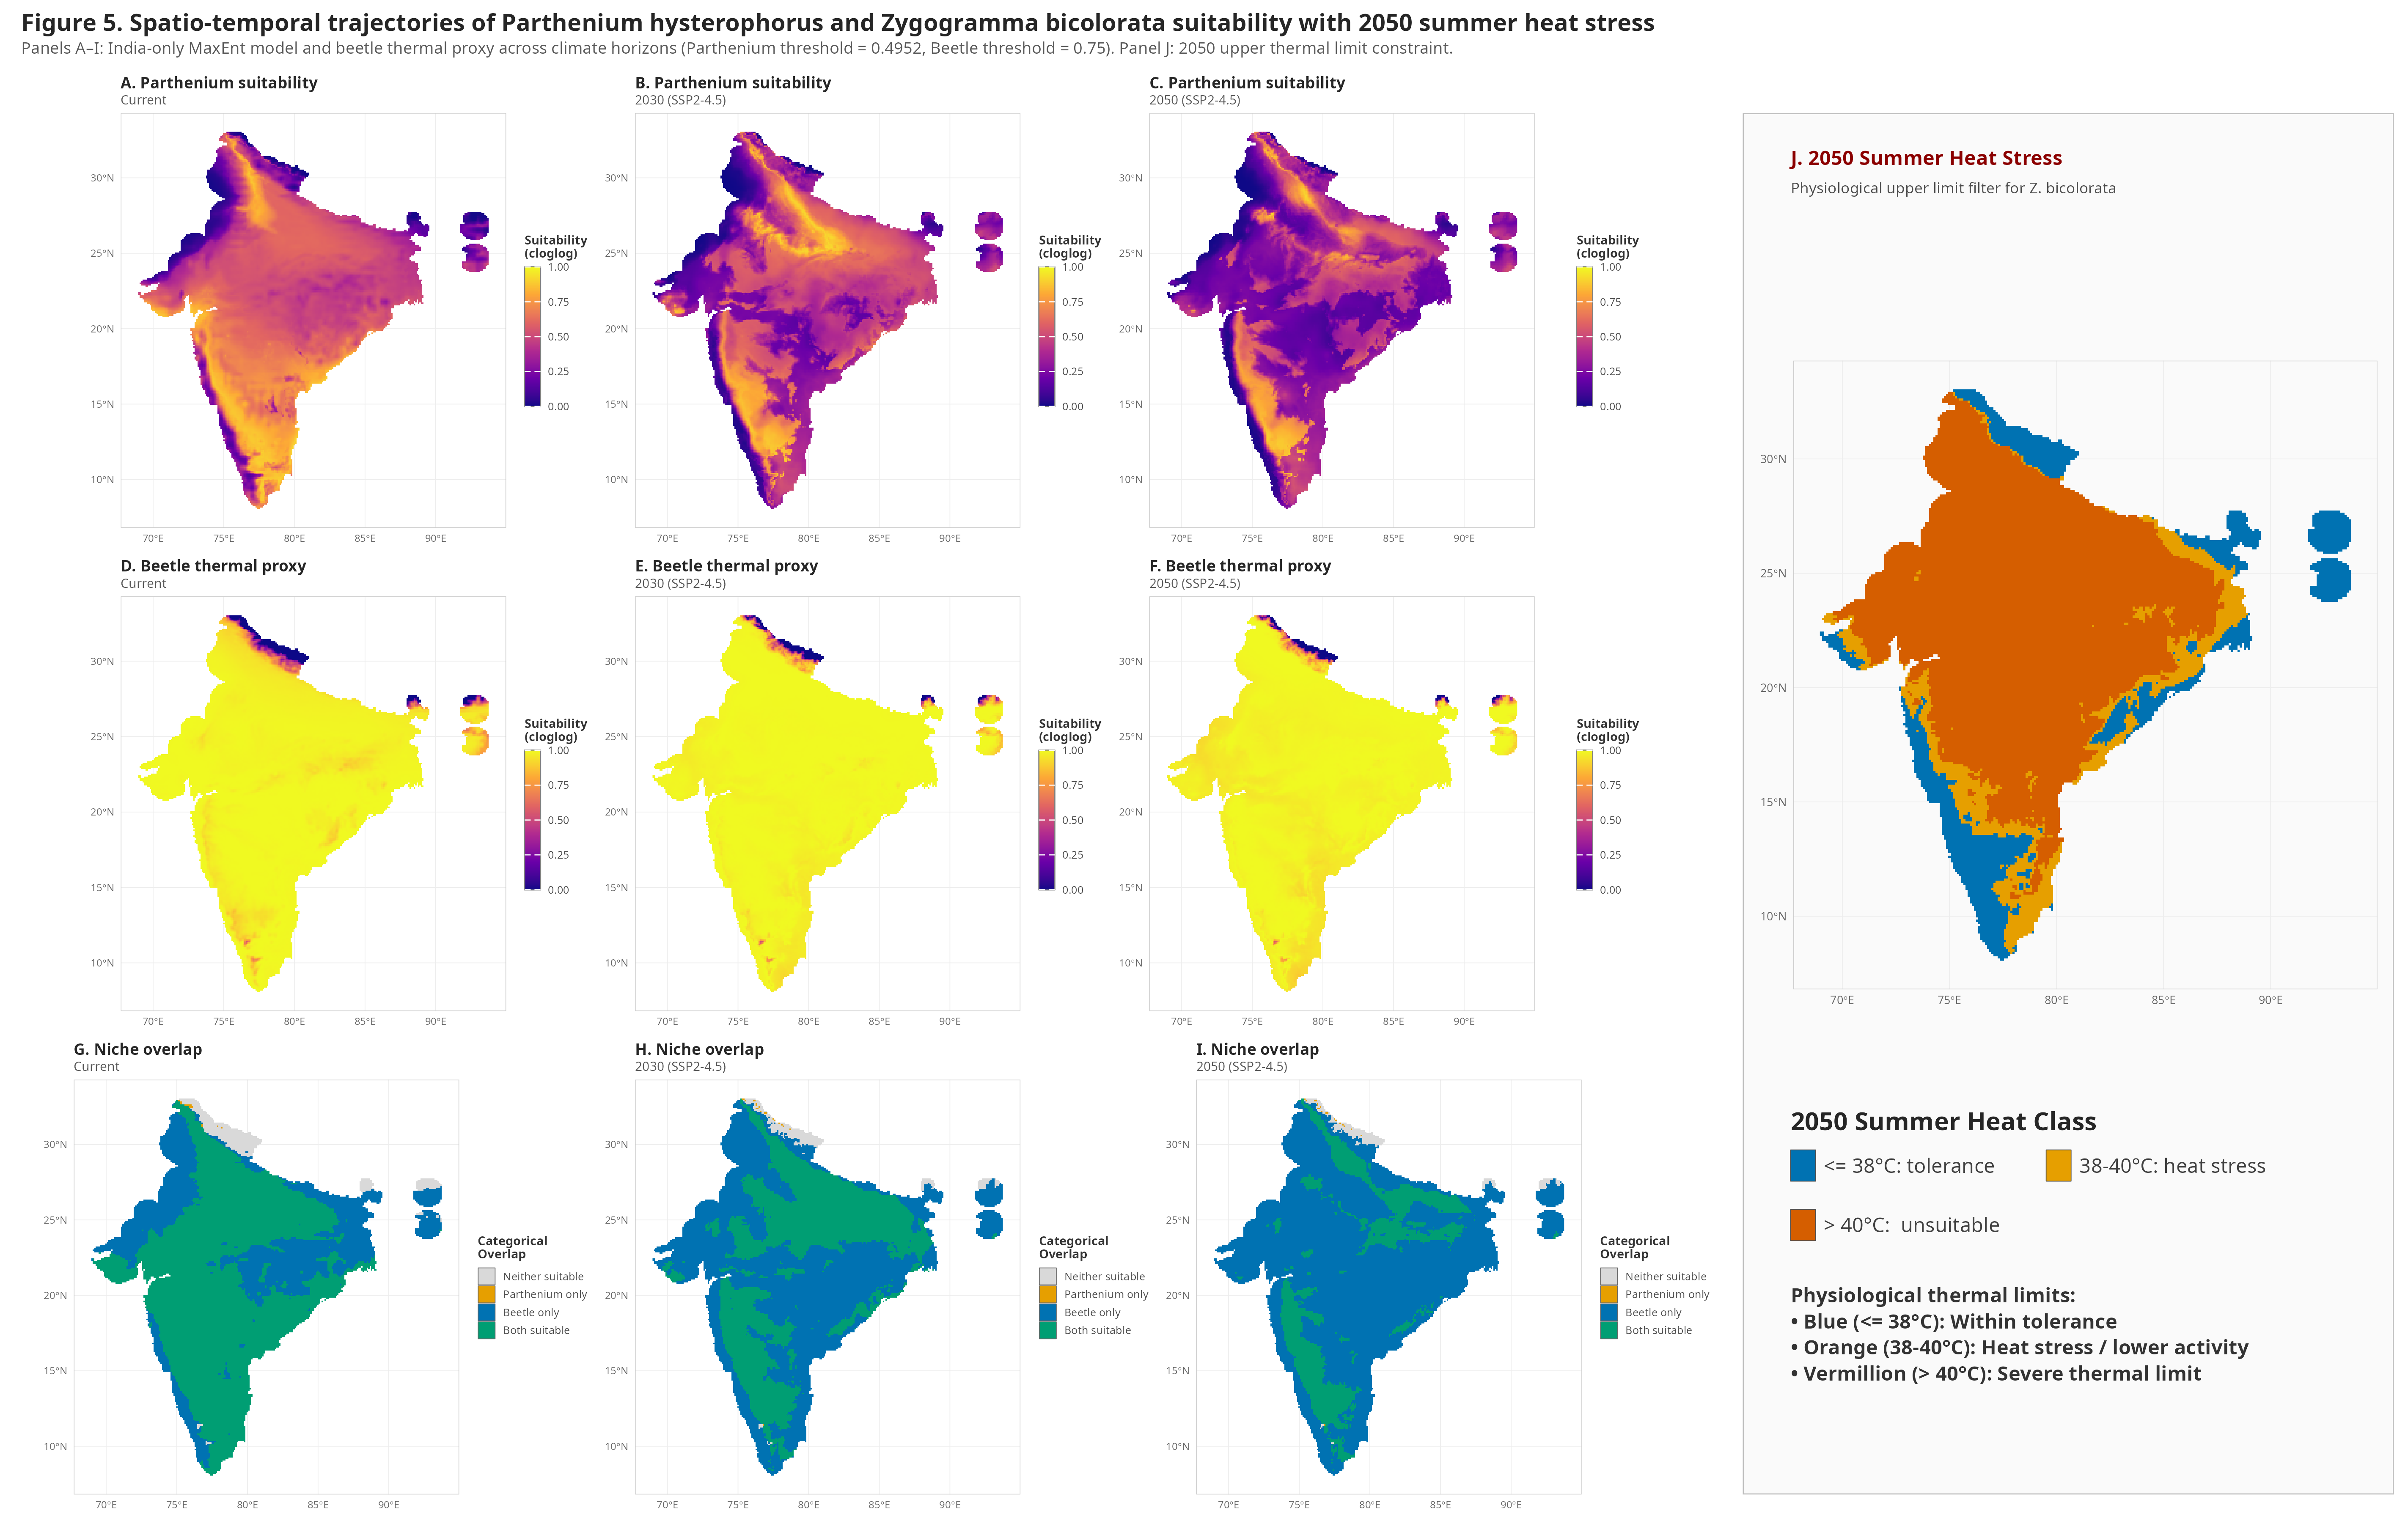
\includegraphics[width=\textwidth]{figures/fig5_india_projections.png}
    \caption{India-only projections of \textit{Parthenium} suitability, beetle thermal suitability, overlap, and supporting 2050 summer heat stress. Panels A--C show climatic suitability for \textit{Parthenium hysterophorus} predicted from the India-only MaxEnt/maxnet model for the current period, 2030, and 2050. Panels D--F show a thermal suitability proxy for the beetle based on annual mean temperature using a temperature-response function with Tmin = 10$^{\circ}$C, Topt = 27$^{\circ}$C, and Tmax = 38$^{\circ}$C. Panels G--I show categorical overlap between \textit{Parthenium} suitability and beetle thermal suitability, classified using thresholds of 0.4952 for \textit{Parthenium} and 0.75 for the beetle proxy. Overlap classes indicate areas suitable for neither, \textit{Parthenium} only, beetle only, or both. The supporting panel (J) shows 2050 maximum summer temperature classified according to beetle upper thermal limits: $\leq 38^{\circ}$C = within broad tolerance, 38--40$^{\circ}$C = heat stress, and $> 40^{\circ}$C = likely unsuitable for sustained summer survival. The beetle layer should be interpreted as a broad climatic thermal proxy rather than a separate occurrence-based species distribution model.}
    \label{fig:india-projections}
\end{figure}

\section{Spatial model comparison}

A comparison of spatial projections from the Pakistan-calibrated GAM and the India-calibrated MaxEnt models revealed only partial concordance across Pakistan (Figure~\ref{fig:pakistan-concordance}). Analysis of 7{,}246 overlapping grid cells revealed a weak association (Spearman's $\rho = 0.295$; Pearson's $r = 0.143$). Both models captured broad spatial trends but differed substantially in location-specific suitability.

The two continuous suitability surfaces showed broadly different spatial structures (Figure~\ref{fig:pakistan-concordance}A--B). The GAM identified southern and south-eastern Pakistan as most suitable, with suitability declining northward. MaxEnt also favoured southern Pakistan but showed greater heterogeneity, with high suitability extending into western and central areas. Both models showed a south-to-north decline, but MaxEnt emphasised more internal spatial variation.

Model agreement on the hotspot areas of predicted suitability was modest, suggesting only a quarter of top-suitability cells overlapped (Jaccard index = 0.251; Figure~\ref{fig:pakistan-concordance}C). Shared high-suitability zones clustered in southern Pakistan (notably the lower Indus), while the GAM highlighted the southern and south-eastern lowlands and MaxEnt emphasised the west and south-west.

The continuous rank-difference surface (Figure~\ref{fig:pakistan-concordance}D) confirmed spatially structured disagreement. Cells ranked higher by the GAM clustered in the south and east, while those favoured by MaxEnt were in the west and central Pakistan. These patterns indicate that the models were not simply differing in prediction intensity, but were prioritising different regions of environmental space when projected across Pakistan.

In summary, the MaxEnt and GAM models captured some broad-scale suitability patterns but showed limited agreement on high-suitability areas. Model choice and calibration geography strongly influence projected suitability, affecting transferability and spatial prioritisation.

\begin{figure}[H]
    \centering
    \includegraphics[width=\textwidth]{figures/fig6_pakistan_concordance.png}
    \caption{Spatial concordance between the Pakistan-calibrated GAM and the India-calibrated MaxEnt projection across Pakistan. (A) Relative suitability predicted by the Pakistan-calibrated GAM. (B) Relative suitability predicted by the India-calibrated MaxEnt model projected onto Pakistan. (C) Categorical spatial concordance based on the upper quartile of predictions from each model, showing cells classified as both low, GAM-only high, MaxEnt-only high, or both high. Relative suitability in panels A and B is shown as within-model percentile rank to allow comparison of spatial pattern rather than absolute prediction magnitude. Concordance was calculated from 7{,}246 overlapping cells. (D) Model divergence map highlighting where models disagree most.}
    \label{fig:pakistan-concordance}
\end{figure}